\chapter{Translation}
\label{chap:translation}
In this chapter we explain the techniques developed for translating a CPN model into program source code. The producer-consumer system is used to illustrate each phase of the translation. The translation from CPN models to the target language is divided into five phases. The idea is to move closer and closer to the target language in small steps. Fig.~\ref{fig:translationphases123} illustrates the first three phases of the translation. These phases are independent of the target language, i.e., there are not made any assumptions about the target language. This means that the target language could, e.g., belong to the imperative or the functional language paradigm.

\begin{figure}[h!]
\centering
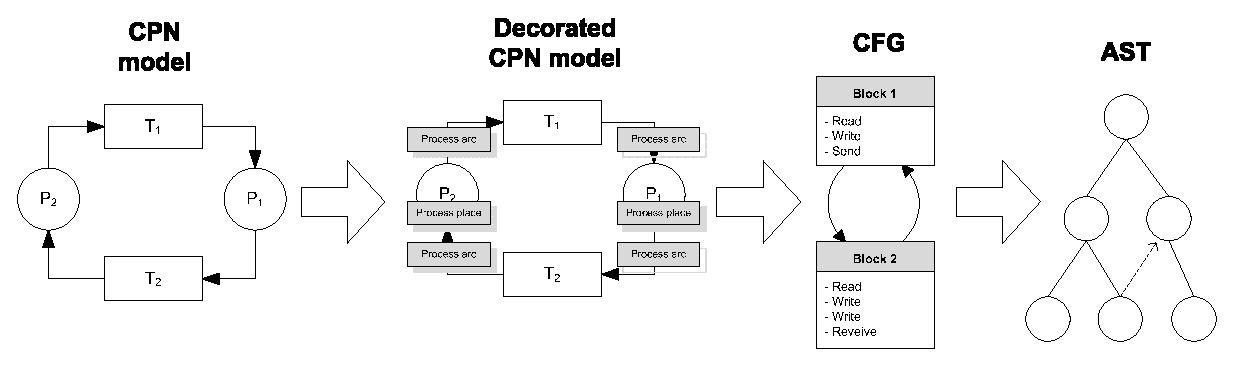
\includegraphics[width=\textwidth]{translation/graphics/phasesfigure01.eps}
\caption{The first three phases of the translation}
\label{fig:translationphases123}
\end{figure}

The first phase consists of decorating the different parts the CPN model with types. The CPN model is assumed to be a ProPCPN model as defined in section \ref{chap:netclass}. The second phase translates from the decorated CPN model into a control flow graph (CFG). A CFG representing the control flow is constructed for each process partition. In the third phase the CFG is translated into an abstract syntax tree (AST) for a simple language. We have designed the language to be abstract enough such that it can be translated into any common type of programming language. The control flow represented by the structure of the CFG is made explicit by, e.g., goto statements in the AST. 

\begin{figure}
\centering
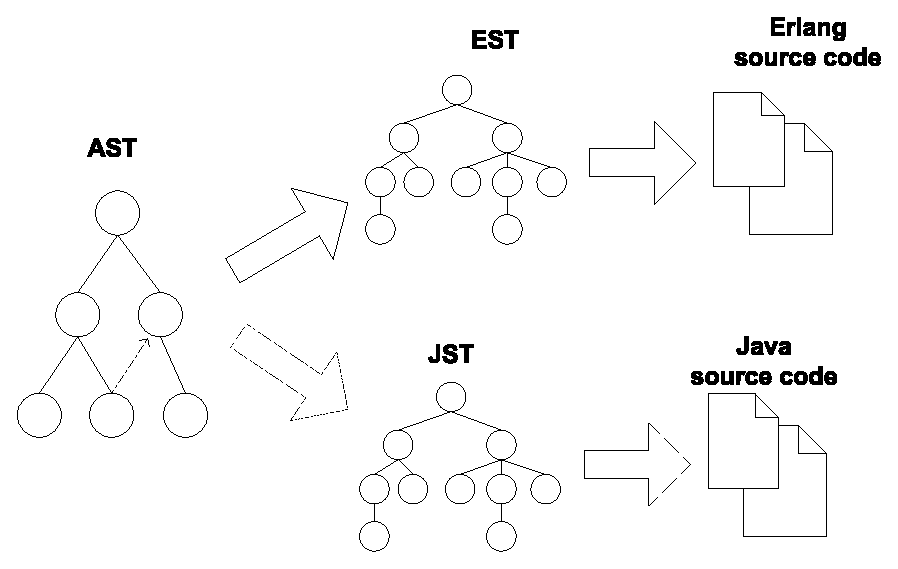
\includegraphics[scale=0.75]{translation/graphics/phasesfigure02.eps}
\caption{The last two phases of the translation}
\label{fig:translationphases45}
\end{figure}

The last two phases of the translation are illustrated in Fig.~\ref{fig:translationphases45}. These phases are language dependent, i.e., the phases are designed for a specific programming language. In Fig.~\ref{fig:translationphases45} two possible target language are illustrated. In the top of the figure, the AST is translated into an Erlang syntax tree (EST) and then into Erlang source code. In the bottom of the figure, the AST is translated into a Java syntax tree (JST) and then into Java source code. We have choosen Erlang as the target language, thus the AST is translated into an EST. The EST can then be transformed into a textual representation by traversing it and printing the nodes according to the Erlang grammar.

\section{Phase 1: Decorating the CPN Model}
\label{sec:cpntodcpn}
The purpose of this phase is to identify different parts of the CPN model and decorate them with a type. This is done in order to simplify the translation from the CPN model to the CFG. This phase uses properties of the ProPCPN net class to perform the identification.

\subsection{Finding Process Partitions}
This phase assumes that the CPN model is a ProPCPN model. When a ProPCPN model is decorated the first thing that needs to be done is to divide it into \emph{process partitions}, i.e., for every node and arc identify which process partition they belong to and decorate them with this information. This is done by using the information provided by the declarations in the ProPCPN model. A process partition is defined with an index colour set declaration which has \code{declare pid} attached to it. The producer-consumer model contains the following declaration:

\begin{verbatim}
colset PRODUCER = index p with 1..2 declare pid;
\end{verbatim}
 
This declaration is an index colour set declaration with a range from 1 to 2, and it has \code{declare} \code{pid} attached. The definition of ProPCPNs defines this to be a process partition named \code{PRODUCER}. The \emph{process variable} related to the process partition is a variable declaration with the type \code{PRODUCER}. In the producer-consumer model we find the declaration:

\begin{verbatim}
var prod : PRODUCER;
\end{verbatim}

This declaration is a variable declaration with the variable name \code{prod} of type \code{PRODUCER}. According to the definition this is a process variable of the \code{PRODUCER} process partition. Analogously, declared index colour set and variable can be found for the \code{CONSUMER} process partition.

\subsection{The Steps of the Decoration}
To illustrate how decorating works for the producer of the producer-consumer system we have decorated the model with labels specifying what type a place or an arc has. The decoration has six steps which are presented in turn.

\begin{description}
\item[Step 1] In this step all \emph{process places} are decorated with the process place type and the corresponding process partition. This is done using the assumption from the definition that only process places have the process type as colour set. Both the \code{PRODUCER} and the \code{CONSUMER} process partitions have two process places, e.g., the places \figitem{Producing} and \figitem{Sending} are labelled as process places for the \code{PRODUCER} process partition since they have the type \code{PRODUCER}. The decoration of the producer process partition can be seen in Fig.~\ref{fig:decoratedproducerconsumerprocessplaces}.

\begin{figure}[h!]
\centering
\includegraphics[width=\textwidth]{translation/cpn_to_dcpn/graphics/decorated_model_process_places.eps}
\caption{The producer decorated with process places}
\label{fig:decoratedproducerconsumerprocessplaces}
\end{figure}

\item[Step 2] The \emph{transitions} in the model are decorated with the process partition they belong. According to the definition, it is only allowed for transitions to move process tokens from its own process partition. Furthermore, a transition must move at least one process token, thus the process partition of the connected process places determine the process partition of the transition. The transitions \figitem{ProduceData} and \figitem{SendData} are both connected to process places from the \code{PRODUCER} process partition and therefore these transitions belong to this partition.

\item[Step 3] Then, \emph{local places} are identified. The definition specifies that for a place to be a local place it must only be connected to transitions from a single process partition. A local place also has the product colour set, where the first component is a process type, and the second component is a data. Since all transitions already have been decorated with their process partition, the task is to look at places with the above mentioned colour set and check that the transitions connected to that place all belong to the same process partition. The producer-consumer model has three local places, namely \figitem{Data}, \figitem{ProducedData} and \figitem{ReceivedData}. These are local places because they have a colour set of the correct form, and they are only connected to transitions from one process partition. The decoration of the producer process partition with local places, buffer places, and shared places can be seen in Fig.~\ref{fig:decoratedproducerconsumerotherplaces}.

\begin{figure}[h!]
\centering
\includegraphics[width=\textwidth]{translation/cpn_to_dcpn/graphics/decorated_model_other_places.eps}
\caption{Decoration with local places, a buffer place, and a shared place}
\label{fig:decoratedproducerconsumerotherplaces}
\end{figure}

\newpage

\item[Step 4] Next, the \emph{buffer places} are decorated. They have colour sets on the same form as local places, but they are connected to transitions from more than one process partition. The place \figitem{Buffer} is the only buffer place in the model.

\item[Step 5] The last places to be identified are \emph{shared places}. They are the only places which have a non-process colour set, and that are not a pair with a process identifier. The place \figitem{NextConsumer} is identified as a shared place because the colour set of this place is not a product and not a process type.

\item[Step 6] In the final step of the decoration the \emph{arcs} are decorated. Arcs are decorated according to the type of place they are connected to, e.g., the arcs connected to the local place \figitem{Data} are local arcs. Similar the arc from \figitem{ProduceData} to \figitem{Sending} is a process arc. The decoration of the producer process partition with arc types can be seen in Fig.~\ref{fig:decoratedproducerconsumerallarcs}.
\end{description}

\begin{figure}[h!]
\centering
\includegraphics[width=\textwidth]{translation/cpn_to_dcpn/graphics/decorated_model_all_arcs.eps}
\caption{The producer-consumer CPN model decorated arc types}
\label{fig:decoratedproducerconsumerallarcs}
\end{figure}

After these steps, all nodes and arcs in the CPN model have been decorated. The model is now ready to be translated from a CP-net into a control flow graph.

\section{Phase 2: Translating the Decorated CPN Model to a CFG}
\label{sec:dcpntocfg}
The main purpose of this phase is to extract the control flow from the decorated CPN model and make it explicit in a control flow graph (CFG). This phase also identifies common program constructs, e.g., processes, variable, and access to variables. Furthermore, the phase finds synchronisation points, i.e., messages passing between processes. The CFG we use is a directed graph in which arcs correspond to control flow and nodes corresponds to a sequence of statements to be executed.

\subsection{Performing the Translation}
\label{sec:cpntranslation}
Given the decorated CPN model belonging to the class ProPCPN, this phase translates it into a CFG. With the decorated CPN model it is straightforward to operate on a model from a process partition perspective, e.g., to iterate through all process places in a given process partition. A CFG is constructed for all process partition in the model, thus in the producer-consumer system two CFGs are generated: one for the \code{producer} process partition and one for the \code{consumer} process partition. In Fig.~\ref{fig:prodconscfg} we see the translated CFG for the \code{producer} process partition. Below we explain how it is obtained from the decorated ProPCPN model.

\begin{figure}[b!]
\centering
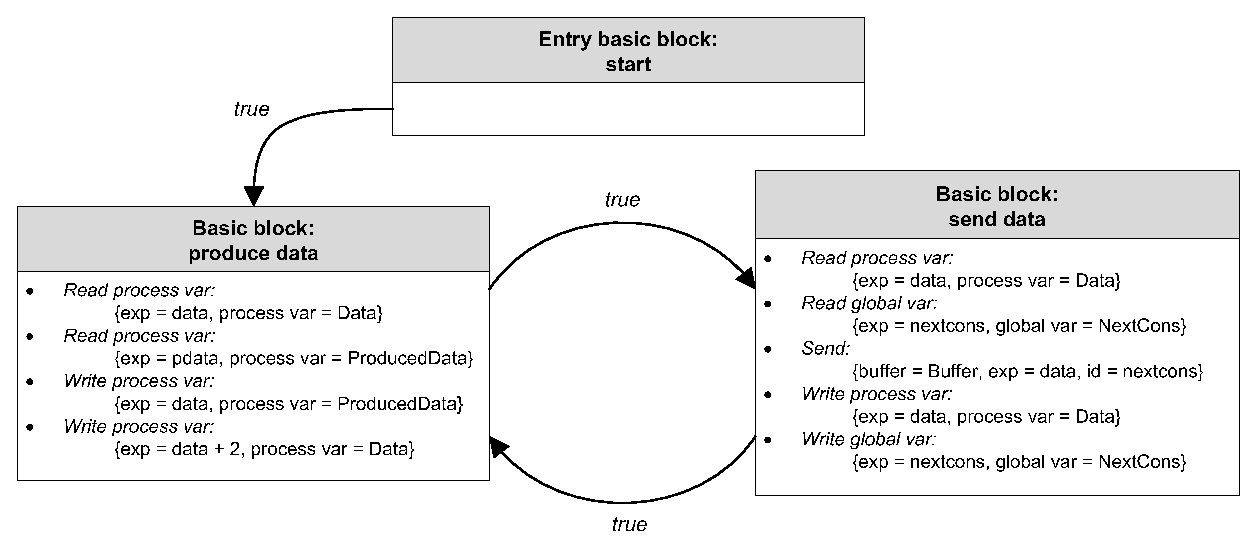
\includegraphics[width=\textwidth]{translation/dcpn_to_cfg/graphics/producerconsumercfg.eps}
\caption{The CFG of the producer process}
\label{fig:prodconscfg}
\end{figure}

%The initial state of each process instance is extracted form the initial marking of the process partition. This information is carried along in the variables for each process partition in the CFG.  \fxnote{maybe move this to another place?}

\subsubsection{Local Places}
In the CPN model, process instances use local places to store data. In a programming language this corresponds to reading/writing a variable, thus a local place is translated into a CFG \emph{process variable}. The name process variable indicates that the scope of these kinds of variables is within a given process. The \code{producer} process partition contains the two process variables \code{Data} and \code{ProducedData} corresponding to the two local places \figitem{ProducedData} and \figitem{Data} in the CPN model. 

Since a local place has an initial marking it is important to carry along this information in the corresponding process variable. The initial expressions for the variables are extracted from the initial markings of the local places. In the producer-consumer system the initial marking of the local place \figitem{ProducedData} is empty, thus the initial expression of the corresponding process variable contains the empty expression. The CFG variable node \code{Data} contains two initial expressions for the two \code{producer} process instances. In general, a process variable contains an initial expression for each process instance. 


\subsubsection{Buffer Places}
In a ProPCPN model, process instances use buffer places to share data with a particular process instance. In a programming language this corresponds to sending to and receiving from a buffer, thus a buffer place is translated into a \emph{buffer} in the CFG. In the producer-consumer system there is one buffer corresponding to the buffer place \figitem{Buffer}.


\subsubsection{Shared Places}
Process instances use shared places in the CPN model to share data with multiple process instances. In a programming language this corresponds to a global variable or some shared memory where process instances can share data. Shared places are therefore translated into \emph{global} variables in the CFG. In the producer-consumer system there is one global variable corresponding to the shared place \figitem{NextConsumer}. The initial marking of the shared place is extracted and carried along in the global variable. 

\subsubsection{Transitions}
Transitions in the CPN model are translated into \emph{basic blocks} in the CFG. In the producer process partition (see Fig. \ref{fig:prodconscfg}) the transition \figitem{ProduceData} is translated into the basic block \code{produce data} and the transition \figitem{SendData} is translated in the basic block \code{send data}. An item in a basic block in Fig.~\ref{fig:prodconscfg} should be read as follows: the name of the statement is written in italic, and the body of the statement is written in curly brackets. 

The basic block is constructed from the input and output arcs to and from the transition. Arcs are translated depending on the type of the arc. In the decorated CPN model, the connected arcs are labelled with types. In the following we consider arcs connecting transitions to local places, shared places, and buffer places.

\paragraph*{Arcs connecting a transition to a local place.}
An input arc with a arc expression on the form \code{(pid, var)} from a local place to a transition corresponds to process instance \code{pid} reading a variable \code{var}. Consider the input arc expression \code{(prod, data)} from the local place \figitem{Data} to the transition \figitem{ProduceData}. This arc is translated to a \emph{Read process var} with the expression \code{data} as shown in Fig.~\ref{fig:prodconscfg}. The \emph{Read process var} also has a pointer to the process variable \code{Data} since this is where it gets its input from.

An output arc expression on the form \code{(pid, exp)} from a transition going to a local place corresponds to process instance \code{pid} writing an \code{exp} to a variable \code{var}. Consider the output arc expression on the arc from the transition \figitem{ProduceData} to the local place \figitem{ProducedData}. This is translated to a \emph{Write process var} (seen in Fig.~\ref{fig:prodconscfg}) containing the expression \code{data} which is extracted from the CPN model. The \emph{Write process var} has a pointer to the variable \code{ProducedData} since this is where the value should be written to.

\paragraph*{Arcs connecting a transition to a buffer place.}
An input arc with the arc expression \code{(pid, var)} from a buffer place to a transition corresponds to a process receiving a message which is put into a variable \code{var}. This kind of input arc can be found in the consumer part of the producer-consumer system on the input arc (with the expression \code{(cons, data)}) from the buffer place \figitem{Buffer} to the transition \figitem{ReceiveData}. This is translated into a \emph{receive} which has the expression \code{data} meaning that the value of the received data should be read into the variable \code{data} for later use. 

An output arc with the arc expression on the form \code{(pid, exp)} from a transition to a buffer place corresponds to sending an expression \code{exp} to a process instance \code{pid}. Consider the output arc expression \code{(nextcons, data)} from the transition \figitem{SendData} to the buffer place \figitem{Buffer}. As seen in Fig.~\ref{fig:prodconscfg} this is translated a \emph{send} which points to the CFG \emph{buffer}. It contains the expression \code{data} and the receiver process instance \code{nextcons}.

\paragraph*{Arcs connecting a transition to a shared place.}
An input arc with the arc expression \code{var} from a shared place to a transition corresponds to a process reading a variable with a global scope, i.e., a variable that can be accessed and modified by multiple process instances. 

In the producer-consumer system there is a input arc expression \code{nextcons} to the transition \figitem{SendData} from the shared place \figitem{NextConsumer}. As seen in Fig.~\ref{fig:prodconscfg} this is translated to a \emph{Read global var} which points to the global variable \code{NextConsumer} and contains the expression \code{nextcons}. 

An output arc with the arc expression \code{var} from a transition to a shared place corresponds to a process writing to a global variable. Consider the output arc expression to the transition \figitem{SendData} from the shared place \figitem{NextConsumer}. This is translated to a \emph{Write global var} which points to the global variable \code{NextConsumer} and contains the expression \code{nextcons}.

\subsubsection{Process Places}
Process places in the CPN model are not explicitly translated into nodes in the CFG, but instead represented as edges between basic blocks. The idea is, for each basic block, to have a set of reachable basic blocks. In Fig.~\ref{fig:prodconscfg} we see that the basic block \code{produce data} has an edge to \code{send data} which means that after executing \code{produce data} the control should flow to the basic block \code{send data}. The condition \code{true} on the edge indicates that it is an unconditional flow of control. There is a special \emph{entry} basic block for each CFG that represent the starting point of the program. In Fig.~\ref{fig:prodconscfg} it points to the basic block \code{produce data}. In section \ref{sec:advancedissues} we explain how conditional flows are handled.

\subsection{The Structure of the Control Flow Graph}
\label{sec:cfgebnf}
A CFG is created for each process in the program, e.g., one CFG for the \code{producer} process and one for the \code{consumer} process. The CFG is a directed graph where the nodes in the graph are connected by labelled edges. The nodes in the graph represent the basic blocks and the edges represent the control flow between the blocks. The labels on the edges are \emph{conditions}, i.e., a list of boolean expressions, specifying whether the control flow can follow this edge or not.

The CFG contains a special entry basic block which is always the starting point for the control flow. The entry basic block only has outgoing edges because the control is never supposed to return to the entry point. 

The basic blocks in the CFG contains a collection of statements, e.g., read, write, send, and receive statements. Taking a closer look at, e.g. read statements, we can see that they contain a pointer to a process variable and an expression. The expression specifies a local variable that the value of the process variable is to be read into.

\section{Phase 3: Translating the CFG to an AST}
\label{sec:cfgtoast}
The main purpose of this phase is to take the control flow given in the structure of the control flow graph (CFG) and translate it into a tree form consisting of nodes representing common programming constructs, e.g., jump statements. Furthermore, read and write expressions contained in the CFG are parsed and translated into subtrees in order to make the there structure explicit in the produced tree.

\subsection{Performing the Translation}
The tree this phase produces is an abstract syntax tree (AST) for a simple language that contains common program constructs, e.g., jump statements, read and write statements and conditional statements. The AST contains a node for each program construct. The root node is a \emph{program node} that contains a number of \emph{processes} and \emph{global variables}. A process has a number of \emph{blocks}. This is the basic structure of the AST and to explain the translation we look at how the CFG for the producer-consumer system is translated into an AST. Fig.~\ref{fig:producerast} shows a subtree of the AST where only the nodes from the \code{produce data} block of the \code{producer} process is shown.

\begin{figure}
\centering
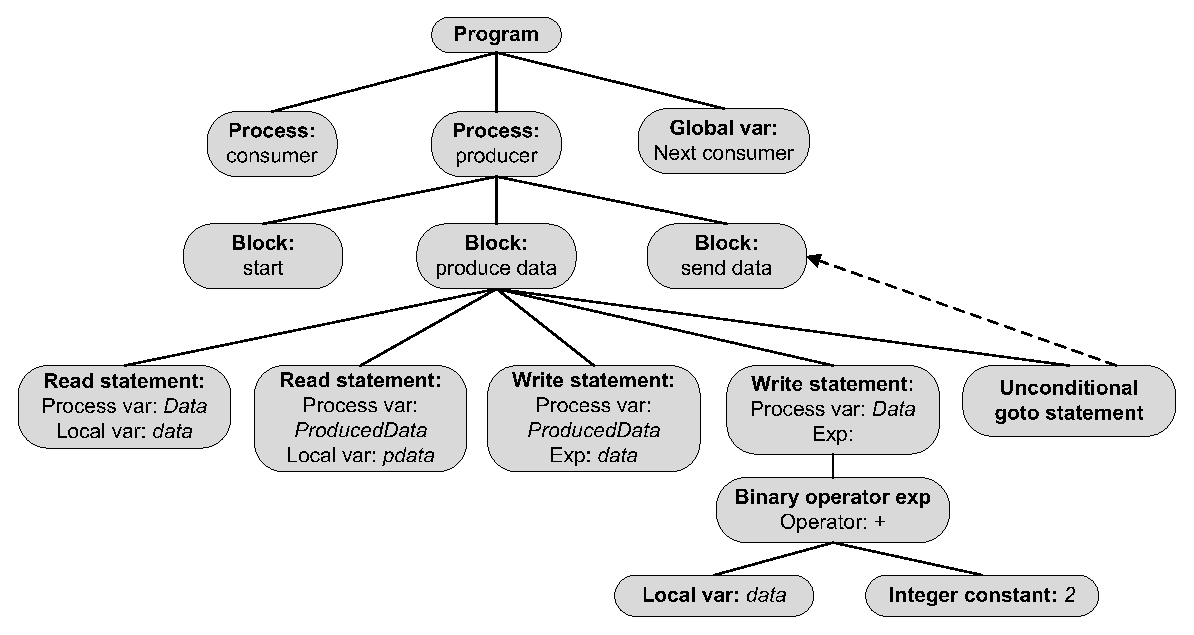
\includegraphics[width=\textwidth]{translation/cfg_to_ast/graphics/producerast.eps}
\caption{The AST for the "produce data" part of the producer}
\label{fig:producerast}
\end{figure}

When building the AST a process is created for each CFG process. As Fig.~\ref{fig:producerast} shows the program contains two processes, namely the \code{producer} and the \code{consumer}. The program node also contains the global variable \code{NextConsumer}. In the CFG each process contains a number of variables. These variables are translated into process variables local to each process. A process variable contains an initial expression for each instance of the process. Each initial expression is parsed and if not recognised an unknown expression is inserted. An AST process also has a number of AST blocks which are created from the basic blocks of the CFG. The \code{producer} process contains three blocks: \code{produce data}, \code{send data}, and \code{start}. Below, we explain how the block \code{produce data} is created.

\paragraph*{Read statements.} The first two child nodes in the \code{produce data} block are \emph{read statements}. These are translated from the two readings in the CFG of the process variables \code{Data} and \code{ProduceData}, respectively. A read statement contains both a \emph{local variable} and a \emph{process variable}. A local variable is a variable that is local to the block, and a process variable is local to the process. The value of a process variable is read into a local variable, e.g., the first read statement reads the value of the process variable \code{Data} into the local variable \code{data}.

\paragraph*{Write statements.} The next two nodes of the block are \emph{write statements} which write values to process variables. These are translated from the two writings in CFG to the process variables \code{ProduceData} and \code{Data}, respectively. Write statements contain an expression which becomes the new value of the process variable. The expression can, e.g., be the value of a local variable or an arithmetic expression.

The first write statement writes the value of the local variable \code{data} to the process variable \code{ProducedData}. The second write statement writes a value the process variable \code{Data}. This value is a binary operator expression which on the left hand side has the value of the local variable \code{data} and on the right hand side the integer constant \code{2}. This expression shows an example of how the structure of expressions are represented in the AST.

\paragraph*{Goto statements.} The rightmost node in the \code{produce data} block is an \emph{unconditional goto statement} which is a jump statement without a condition. It has a pointer to the block it jumps to which in this case is the \code{send data} block. The jump statements are translated from edges between basic blocks in the CFG. An AST has two types of goto statements, namely a unconditional without a condition, and a conditional which has a condition attached to it. The condition is a boolean expression specifying whether the jump should be made or not. Common for both types is that they have a pointer to an AST block which is the target of the goto statement.

\begin{figure}[b!]
\centering
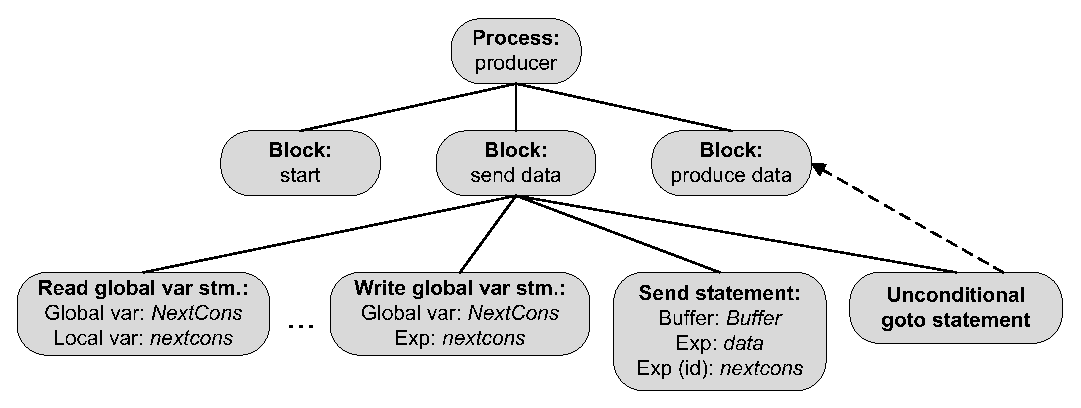
\includegraphics[scale=0.7]{translation/cfg_to_ast/graphics/producersendast.eps}
\caption{The AST for the "send data" part of the producer}
\label{fig:producersendast}
\end{figure}

\paragraph*{Read and write to and from global variables.}
Fig.~\ref{fig:producersendast} shows the "send data" part of the \code{producer} process. The three dots between the two first nodes indicates that we have left out a read and a write statement which reads the value of the process variable \code{ProducedData} into the local variable \code{data} and writes the same value back to \code{ProducedData} leaving it unchanged.

The first node in the \code{send data} block is a \emph{global variable read statement} which reads the value of the global variable \code{NextCons} into the local variable \code{nextcons}. This is very similar to a read statement from a process variable. The read statements of global variables are translated from the readings of global variables in the CFG.

The \emph{global variable write statements} are translated from writings of global variables from the CFG and are also very similar to writings to process variables. The second node in Fig.~\ref{fig:producersendast} writes the value of the local variable \code{data} to the global variable \code{NextCons}.

\paragraph*{Send statements.} The third node in the \code{send data} block is a \emph{send statement}. A send statement contains a pointer to the buffer that is to receive the message, and an expression that specifies the process identifier of the receiving process. With this information, a process is able to send a message to a specific buffer for a specific process. A send statement also contains an expression which specifies the value which is sent.

Send statements are translated from the send statements in the CFG. In Fig.~\ref{fig:producersendast} the send statement is to send the value of the local variable \code{data}, which was read from the process variable \code{ProducedData}. This value should be send to the buffer \code{Buffer} for the process which is identified by the value of \code{nextcons}, that was read from global variable \code{NextCons}.

\paragraph*{Receive statements.} Messages are received using a \emph{receive statement}. A receive statement has a pointer to a buffer where the incoming messages are stored and where the process can read the messages from. It also contains a local variable into which a message from the buffer is read. The receive statements are translated from the receive statements in the CFG. An example of the use of a receive statement is found in the \code{consumer} process when it receives the produced data from a \code{producer} process.

\subsection{The Structure of the AST}
% Forklar EBNF

\begin{figure}[b!]
\footnotesize
\begin{verbatim}
<Program>                    ::= *<Process> *<GlobalVariableDeclaration>
<GlobalVariableDeclaration>  ::= <Name> <InitialExpression>
<Process>                    ::= <Name> *<Block> <EntryBlock> 
                                        *<ProcessVariableDeclaration>
<Name>                       ::= string
<ProcessVariableDeclaration> ::= <Name> <InitialExpression>
<InitialExpression>          ::= <Expression>
<Block>                      ::= <Name> <Statements>
<EntryBlock>                 ::= <Block>
<Statements>                 ::= *<Statement> |
                                 <Statements> <UnconditionalGotoStatement>
<Statement>                  ::= <LocalVariableDeclaration> |
                                 <ReadStatement> | <ReceiveStatement> |
                                 <GlobalVariableReadStatement> |
                                 <WriteStatement> | <SendStatement> |
                                 <GlobalVariableWriteStatement> |
                                 <ConditionalGotoStatement>
...
<Expression>                 ::= <BinaryOperatorExpression> |
                                 <LocalVariableExpression> |
                                 <GlobalVariableExpression> |
                                 <ProcessVariableExpression> |
                                 <UnknownExpression> |
                                 <IntegerConstantExpression> |
                                 <StringExpression> | <Undefined>
...
\end{verbatim}
\normalsize
\caption{The EBNF for the abstract syntax tree}
\label{fig:ASTEBNF}
\end{figure}


In order to explain the structure of the AST more precisely we describe it using the Extended Backus-Naur Form (EBNF) \cite{EBNF}. Part of it is shown in Fig.~\ref{fig:ASTEBNF} and the full version can be found in appendix \ref{app:astebnffull}. The first definition is a \code{Program} which consists of zero or more processes and zero or more global variable declarations. A \code{GlobalVariableDeclaration} is a declaration of a variable that can be accessed by every running process in the program, i.e., a variable which is shared between processes. The \code{GlobalVariableDeclaration} consists of a name, which is a string, and an initial expression which is used to initialise the global variable.

A \code{Process} has a name which is simply a string. It has zero or more \code{Block}s which is a named block of statements. Furthermore, a \code{Process} has one or more \code{ProcessVariableDeclaration}s which is declarations of variables that can be accessed anywhere within the process. Finally, a \code{Process} has a \code{StartBlock} which is the first block of statements to be executed in the process.

Taking a closer look at the \code{Statement} and \code{Statements} constructions we see that they contain both a \code{ConditionalGotoStatement} and an \code{Unconditional}-\code{GotoStatement} which represents goto statements with or without an attached condition, respectively. The construction is made in such a way that if an \code{UnconditionalGotoStatement} appears there cannot appear other types of statements afterward. This is done to avoid unreachable statements.

The last construction in the EBNF is \code{Expression} which consists of all the types of expressions in the AST. We have chosen only to support a small set of expressions. E.g., we have chosen \emph{Binary Operator Expressions} to illustrate how expressions can be parsed from CPN ML into a tree structure fitting the AST. Other expressions are simply wrapped in an \code{UnknownExpression} which contains the expression as the original string. The type \code{Undefined} is used when, e.g., a variable has no initial value.

\section{Phase 4: Translating the AST to an EST}
\label{sec:astest}

This phase generates an Erlang syntax tree (EST) based on an AST. The purpose of this phase is to translate the abstract representation of a program into an Erlang program represented as a tree. The control flow, represented by goto statements in the AST, is translated into the functional language paradigm equivalent \emph{function calls}. Since functional languages are stateless the state is passed along in the function calls. Processes are native in the Erlang language, thus each process in the AST is simply translated into a module. The generated modules are spawned in a special \emph{system} module.

\begin{figure}[b!]
\centering
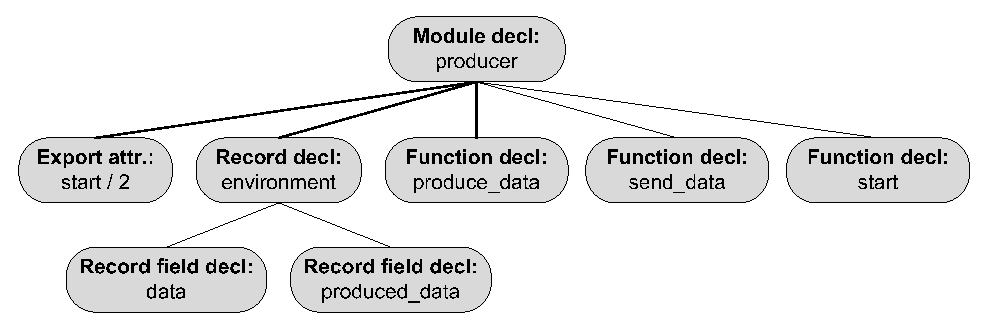
\includegraphics[width=\textwidth]{translation/ast_to_est/graphics/producerest01.eps}
\caption{The producer module of the EST}
\label{fig:prodmoduledecl}
\end{figure}

To give an impression of the translation from an AST to an EST we take a look at the producer-consumer system. Figure \ref{fig:prodmoduledecl} shows how a part of the producer is represented in the generated EST. In the following we explain how this EST and some of its subtrees are created.

\subsection{Performing the Translation}
In this section we first describe how AST processes are translated into EST module declarations. Next, we describe how global variables are translated into modules which can be used to share data among processes. Then we explain how AST blocks are translated into functions, and how a \code{start} function is created in each module. At the end of this section we describe a special system module responsible for spawning process instances.

\subsubsection{Process Nodes in the AST}
For each AST process node we create an EST \emph{module declaration}. Figure \ref{fig:prodmoduledecl} shows the \code{producer} module declaration for the producer-consumer system. AST processes contain process variables which are shared among blocks in that specific process. This kind of variables are not directly supported in Erlang, but by having a dedicated \emph{environment} record which is carried along in the function calls we get the same result as with process variables. For each AST process variable a field with the same name is created in the environment record. In Fig. \ref{fig:prodmoduledecl} we see the record declaration \code{environment}. There are two process variables \code{produced\_data} and \code{data} in the AST, thus the environment contains two \emph{record field declarations} corresponding to \code{produced\_data} and \code{data}.

\subsubsection{Global Variable Declarations}
Global variables in the AST are used to share data between processes. There is no native equivalent to global variables in the Erlang language, but instead we have constructed a module which can be used to spawn processes that acts like global variables. The module we create is identical to the module \code{shared} described in section \ref{subsec:thesharedstore}.

\subsubsection{Block Nodes in the AST}
An AST process contains a number of blocks describing the behaviour of the process. Blocks are translated into \emph{function declarations} in the EST. The \code{producer} module declaration thus contains two function declarations: \code{produce\_} \code{data} and \code{send\_data} as seen in Fig.~\ref{fig:prodmoduledecl}. Fig.~\ref{fig:prodproducefunc} shows the function declaration corresponding to the AST block \code{produce data}. As mentioned earlier the environment is given as argument to each function, thus an EST \emph{variable} \code{Env} is added to the argument list of the function declaration. 

\begin{figure}
\centering
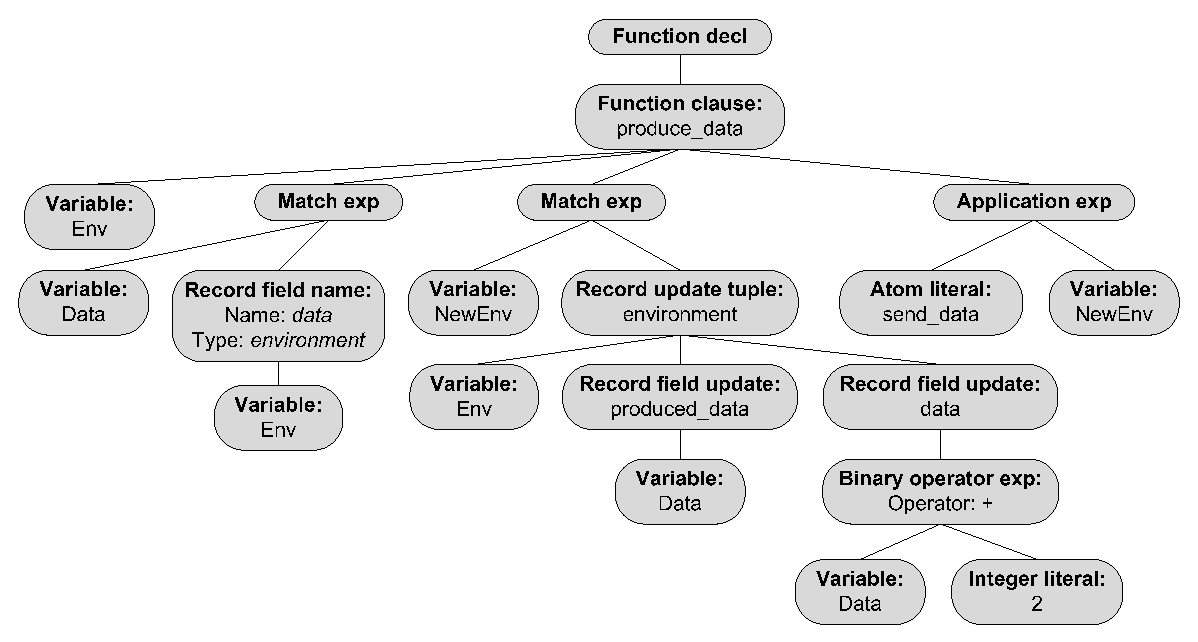
\includegraphics[width=\textwidth]{translation/ast_to_est/graphics/producerest02.eps}
\caption{The function declaration \code{produce\_data}}
\label{fig:prodproducefunc}
\end{figure}

Notice that since the EST is used by phase 5 to print the tree in a depth first traversal, the order of the EST nodes determine the semantic of the resulting Erlang program. Because, e.g., a read variable can be used to update another variable, it is important to do the reading of process variables, reading of global variables and receiving data from buffers, before writing to process variables, writing to global variables or sending data to buffers.

\paragraph*{Read process variable statements.} 
Reading a process variable is done in Erlang by accessing the corresponding field in the environment. In the EST this becomes a lookup in the record for the field with the same name as the process variable. This value is then bound to a variable which has the name given in the local variable expression of the read statement. This can be seen in Fig. \ref{fig:prodproducefunc} where the \emph{record field name expression} with the type \code{environment}, name \code{data}, and the variable \code{Env} is bound to the variable \code{Data}.

\paragraph*{Write process variable statements.}
In Erlang write statements for process variables corresponds to updating the field in the environment for that particular process variable. Fig. \ref{fig:prodproducefunc} shows how this update is represented in the EST. A \emph{record update tuple expression} containing the variable \code{Env} is bound to a variable \code{NewEnv}. The two \emph{record field update}s ensures that the fields \code{data} and \code{produced\_data} are updated corresponding to the write statements to the process variables.

\paragraph*{Receive statements.}
Receiving messages is a native construct in the Erlang language. The received messages are stored in a built-in Erlang buffer. To handle the translation of more advanced control flow constructs (presented in section~\ref{sec:advancedissues}) a buffer with extra functionality is needed. For this reason an explicit \code{buffer} process is used to receive messages. The Erlang code for the \code{buffer} module is found in appendix~\ref{appsec:buffer}. A dedicated buffer process is spawned for each receiving point of each process instance to make it equivalent to using the built-in Erlang buffers. The way to retrieve a message from the buffer is to send the atom \code{get} to the buffer process and the buffer process will send the first message in the buffer back to the requesting process.

Because of the \code{buffer} process, receiving messages it translated into sending a \code{get} request followed by a \emph{receive expression}. In the consumer module we find such an EST (see Fig.~\ref{fig:receiveexp}) in the function clause \code{receive\_data}. It consist of a send expression containing the name of the buffer and the atom literal \code{get}. This is followed by a receive expression with one \emph{receive clause} with the pattern consisting of a variable \code{Data}. The clause body contains one expression, namely the variable \code{Data}. This makes the variable (containing the received data) the return value of the receive expression and thus available in the remaining part of the function.

\begin{figure}[h!]
\centering
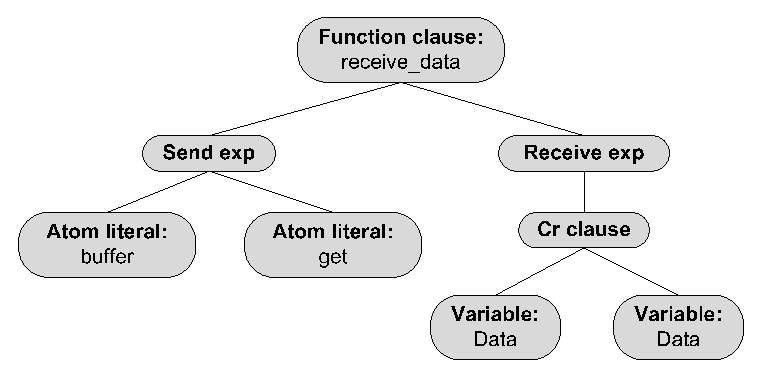
\includegraphics[scale=0.7]{translation/ast_to_est/graphics/producerest03.eps}
\caption{The receive expression subtree of the EST}
\label{fig:receiveexp}
\end{figure}

\paragraph*{Send statements.}
Since message passing is native in the Erlang language this is simply translated into a send expression in the EST. The recipient of the message is given by a buffer and an expression identifying the receiving process. In a send expression the identifier expression evaluates to an integer and together with the buffer it is possible to address the receiver of the message. The send expression furthermore contains an atom literal \code{send} indicating that the message should be added to the buffer. 

\paragraph*{Read global variable statements.}
As explained in section \ref{sec:producerconsumererlang} we have translated global variables into a shared process used to exchange data. Thus reading a global variable is translated to first sending a \code{\{get, id\}} request to the shared process corresponding to the global variable and then receiving some data from the shared process. In Fig. \ref{fig:readglobalvarexp} we see how this works in the \code{send\_data} function of the \code{producer} module. In the EST there is a \emph{send expression} containing the receiver \code{next\_consumer} and a \emph{tuple} containing the atom literal \code{get} and the application expression \code{self()}. An \emph{application expression} is a function call and the Erlang built-in function \code{self()} returns the process ID of the calling process. The send expression is then followed by a receive expression ready to receive the data from the shared process.

\begin{figure}[h!]
\centering
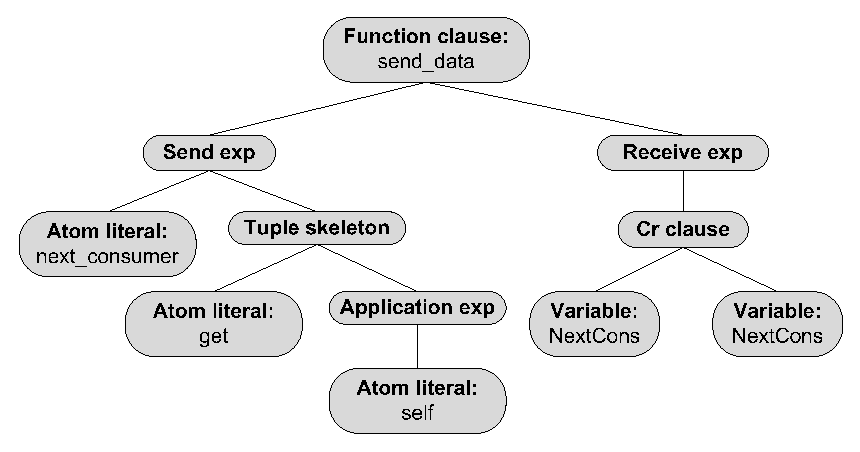
\includegraphics[scale=0.7]{translation/ast_to_est/graphics/producerest04.eps}
\caption{The subtree of the EST reading a global variable}
\label{fig:readglobalvarexp}
\end{figure}

\paragraph*{Write global variable statements.}
In the EST, write statements to global variables are translated into \emph{send expressions} which sends the value to be written to the shared process. The function \code{send\_data} contains a send expression which is a translation of the write statement to the global variable \code{NextConsumer}. This is done by sending a \emph{tuple} containing the atom literal \code{set} and the expression \code{nextcons}.

\paragraph*{Goto statements.}
\emph{Goto} statements in the AST are divided into \emph{unconditional} and \emph{conditional}. Unconditional goto statements are simply translated into application expressions in the EST. In the EST for the function \code{produce\_data} (see Fig.~\ref{fig:prodproducefunc}) we see the application expression containing the atom literal \code{send\_data} and the argument \code{NewEnv}. Conditional goto statements are explained in section \ref{sec:advancedissues}. 


\subsubsection{The Start Function}
The purpose of the \code{start} function is to initialise the environment in the process and call the first function to be executed. The start function takes a number of arguments used to initialise the environment. For each AST process variable an EST variable with the same name as the process variable is added to the function clause argument list. This can be seen in Fig.~\ref{fig:startfunction} showing the \code{start} function in the module \code{producer}. The function clause contains a variable \code{Produced\_data} and a variable \code{Data} as arguments corresponding to the process variable of the same names.  

\begin{figure}[h]
\centering
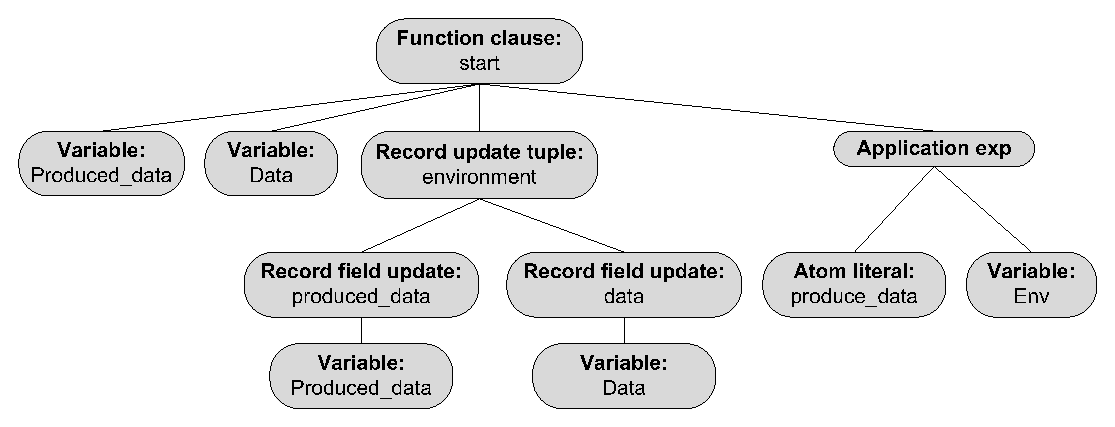
\includegraphics[width=\textwidth]{translation/ast_to_est/graphics/producerest05.eps}
\caption{The subtree of the EST showing the \code{start} function clause}
\label{fig:startfunction}
\end{figure}

The environment is then initialised by creating an environment record where the arguments are used to update to corresponding field. This record is then bound to the variable \code{Env}. In Fig.~\ref{fig:startfunction} this is seen in the match expression where a record update tuple expression is matched to the variable \code{Env}. The record update tuple expression contains two record field update expression: one assigning the variable \code{Produced\_data} to the field \code{produced\_data}, and one assigning the variable \code{Data} to the field \code{data}.

In an AST process there is a entry block which contains a goto statement to the first block to be called. In the EST, an application expression is created calling the function corresponding to the first block. In the \code{producer} module the start function shown in Fig.~\ref{fig:startfunction} calls the function \code{produced\_data}.

The \code{start} function is exported in the module such that it can be called from outside. This can be seen in Fig. \ref{fig:prodmoduledecl} where an \emph{export attribute} exports the \code{start} function taking two arguments.

\subsubsection{Spawning the Process Instances}
We have chosen to have a dedicated module which spawns a process for each process instance. It also spawns the \code{buffer} processes and a \code{shared} process for each global variable. In Fig.~\ref{fig:systemmoduledecl}, the \code{start} function clause of the \code{system} module for the producer-consumer system is shown. It is responsible for spawning process instances, thus in the producer-consumer system this becomes: two producers, two consumers and two buffers belonging to those consumers, and a shared instance. In the \code{start} function clause we find an application expression calling the Erlang built-in function \emph{register} given a name and an application expression calling the Erlang built-in function \emph{spawn}.

\begin{figure}[h]
\centering
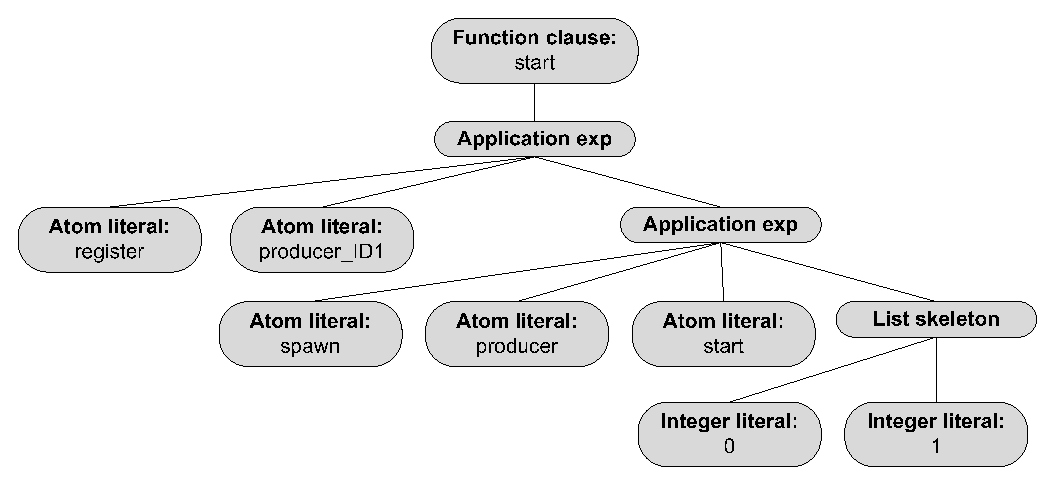
\includegraphics[width=\textwidth]{translation/ast_to_est/graphics/producerest06.eps}
\caption{The function clause \code{start} of the \code{system} module}
\label{fig:systemmoduledecl}
\end{figure}

\subsection{The Structure of the EST}
We describe the EST using EBNF and part of it is shown in Fig.~\ref{fig:ESTEBNF} (the full version can be found in appendix \ref{app:estebnffull}). The EST EBNF is based on the Erlang language specification grammar \cite{RefWorks:91}. The first definition is a \code{Program} which consists of zero or more \code{ModuleDecl}s. A \code{ModuleDecl} has a name, zero or more \code{HeaderForm}s and a \code{ProgramForm}. A \code{HeaderForm} is used to export functions and declare records. A \code{FunctionDecl} consist of a number of \code{FunctionClause}s which contains a function symbol, zero or one \code{pattern} (the arguments to the function clause) and zero or more \code{expression}s (the body of the function clause). A \code{Pattern} is, e.g., an atom literal, or a variable. An \code{Expression} is can be a \code{ApplicationExp}, \code{AtomicLiteral}, \code{BinaryOperatorExp}, \code{MatchExp}, \code{ReceiveExp}, \code{RecordExp}, \code{SendExp}, or a \code{Variable}. An \code{ApplicationExp} contains an expression (which could be an \code{AtomLiteral}) specifying which function to call, and a list of expressions which is the arguments to the function call.
\begin{figure}
\footnotesize
\begin{verbatim}
<Program>              ::= *<ModuleDecl>
<ModuleDecl>           ::= <ModuleName> *<HeaderForm> <ProgramForm> 
<ModuleName>           ::= string
<HeaderForm>           ::= <ExportAttribute> | <RecordDecl>
<ProgramForm>          ::= <FunctionDecl> | 
                           *<ProgramForm> <FunctionDecl> |
                           *<ProgramForm> <RecordDecl> 
<ExportAttribute>      ::= *<FunctionName>
<FunctionDecl>         ::= *<FunctionClause>  
<FunctionName>         ::= <FunctionSymbol> <arity>
<FunctionClause>       ::= <FunctionSymbol> ?<Pattern> *<Expression>
<Pattern>              ::= <AtomicLiteral> | <Variable>
... 
<AtomicLiteral>        ::= string
<Variable>             ::= string
<Expression>           ::= <ApplicationExp> | <AtomicLiteral> |
                           <BinaryOperatorExp> | <MatchExp> | <ReceiveExp> |
                           <RecordExp> | <SendExp> | <Variable> 
...
<ApplicationExp>       ::= <Expression> *<Expression>
<BinaryOperatorExp>    ::= <Expression> <Operator> <Expression>
<MatchExp>             ::= <Pattern> <Expression>
<ReceiveExp>           ::= *<CrClause>
<CrClause>             ::= <Pattern> *<Expression>
<RecordExp>            ::= ?<Expression> <RecordType> <RecordFieldNameExp> |
                           ?<Expression> <RecordType> <RecordUpdateTupleExp>
<RecordFieldNameExp>   ::= <RecordFieldName> 
<RecordUpdateTupleExp> ::= *<RecordFieldUpdate>
<RecordFieldUpdate>    ::= <RecordFieldName> <Expression>
<SendExp>              ::= <Expression> <Expression>
\end{verbatim}
\normalsize
\caption{The EBNF for the Erlang syntax tree}
\label{fig:ESTEBNF}
\end{figure}

\section{Phase 5: Translating the EST to Erlang Code}
\label{sec:esttocode}

The last phase is translating the Erlang syntax tree (EST) into a textual representation. The EST is a concrete representation of Erlang so the task is to traverse the tree, and print a textual representation of each node to a file. The nodes are printed according to a subset of the Erlang grammar \cite{RefWorks:91} which can be found in appendix \ref{app:fullerlanggrammar}. The traversal of the tree is a depth-first traversal. A traversal is made for each module declaration because they represent one text file each. A depth-first traversal starts at the root of the tree which in this case is the module declaration. It then explores as far as possible along each branch before backtracking and exploring the next branch.

The producer-consumer system is used to illustrate how the traversal is performed and Listing~\ref{fig:generatedproducercode} shows a part of the generated Erlang code for the producer module. Fig.~\ref{fig:prodmoduledecl} presented in section~\ref{sec:astest} shows the module declaration of the \code{producer} module along with its children. The traversal starts at the module declaration, which is printed as line 1 in the generated code. Next, the export of the function \code{start} (the first child) is visited, and line 2 is printed. Then the record declaration for the \code{environment} record is visited along with its children, i.e., the two record field declarations for \code{data} and \code{produced\_data}, which prints line 3-5.

\begin{figure}
\begin{verbatim}
- module(producer).
- export([start/2]).
- record(environment, {
 	produced_data,
 	data}).

produce_data(Env) -> 
 	Data = Env#environment.data,
 	NewEnv = Env#environment {produced_data = Data,
 	data = Data + 2},
 	send_data(NewEnv).
\end{verbatim}
\end{figure}

Moving on to the first function declaration (see Fig.~\ref{fig:prodproducefunc} showing the function \code{produce\_data} in the \code{producer} module) we find that it has one clause, namely the function clause named \code{produce\_data}. The function clause has one argument which is the variable child node for the \code{Env} variable. This clause is printed as line 7 in the generated code. The clause node has three other children and the first to be explored is a match expression node. The first child is the left hand side of the expression which is a variable called \code{Data}, and second child is the right hand side which is a record field name that gets the value of the field \code{data} form the variable \code{Env}. This subtree is printed as line 8.

Next, we find another match expression which is similar to the first one, except that here is a record update tuple on the right hand side. This node has two children which are both record field update nodes. One updates the \code{produced\_data} field with the value of the variable \code{Data} and the other updates the \code{data} field with a binary operator expression. The nodes in this subtree are printed as line 9 and 10.

The last child of the function clause node is an application expression node. It has two children, an atom literal \code{send\_data} and a variable node \code{NewEnv}. This application expression node is printed as line 11, i.e., the function call the \code{send\_data} function with the argument \code{NewEnv}.

\section{Advanced Control Flow Issues}
\label{sec:advancedissues}
%In chapter \ref{chap:translation} we described the techniques necessary to generate code from the producer-consumer ProPCPN model. We described in detail how the model was decorated, and then translated into a control flow graph (CFG). The CFG was then translated into an abstract syntax tree (AST) representing a simple language we designed for the purpose. Then we choose the functional language Erlang as the target language, i.e., created an Erlang syntax tree (EST) which could be pretty printed into a textual representation of the program. 

While covering most of the construct found in ProPCP-nets, the producer-consumer model does not contain a branch of the control flow. In this section we describe how branches of control flow are handled in the translation. In the producer-consumer model process tokens residing on a process place are only available to a single transition. The definition allows process tokens to be available to multiple transitions, i.e., a control flow branch. Having control flow branches introduce an additional challenge when the target transitions have input arcs from buffer places. These buffer places have to be taken into consideration when choosing the flow of control. Making a function call without looking at the buffer may introduce a deadlock in the program that did not exist in the model.

\subsection{Control Flow Branches}

\begin{figure}[b!]
\centering
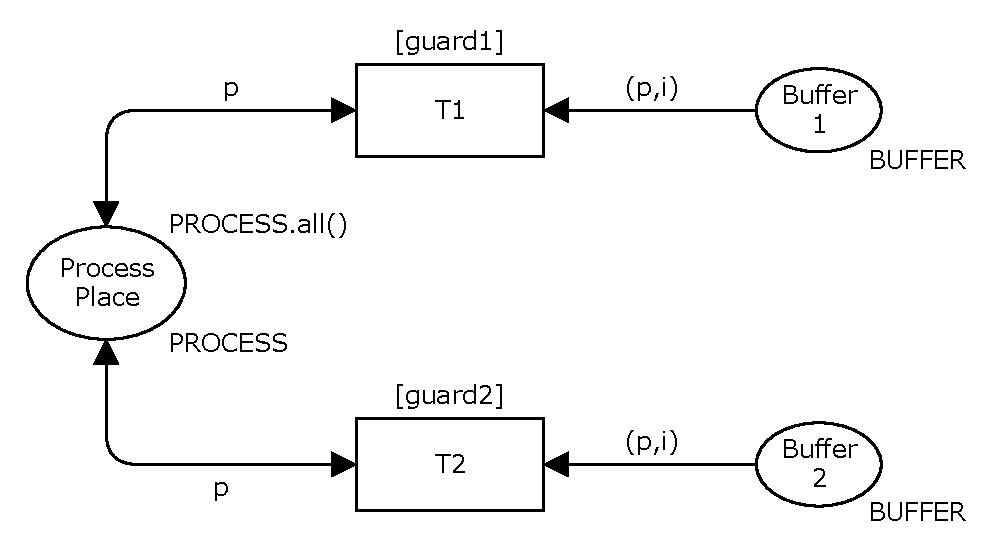
\includegraphics[scale=0.5]{translation/advancedissues/graphics/cffcpn.eps}
\caption{A process partition with a control flow branch}
\label{fig:cffcpn}
\end{figure}

In Fig.~\ref{fig:cffcpn} we see part of a ProPCPN model with one process place \figitem{Process Place}, two transitions \figitem{T1} and \figitem{T2}, and two buffer places \figitem{Buffer1} and \figitem{Buffer2}. The process token can either be removed by \figitem{T1} or \figitem{T2}, and are in both cases, put back on \figitem{Process Place}. \figitem{T1} is enabled if \figitem{guard1} evaluates to \code{true} and there is a token on \figitem{Buffer1}, and analogously for \figitem{T2}. This means that the generated process can proceed to either \figitem{T1} or \figitem{T2} depending on them being enabled.

\subsubsection{Translating to a CFG} 

Given the ProPCPN model shown in in Fig.~\ref{fig:cffcpn} we generate the CFG shown in Fig.~\ref{fig:cffcfg}. It contains an entry basic block \code{start} which has an edge with the condition \code{guard1} to the basic block \code{T1}, and an edge with the condition \code{guard2} to the basic block \code{T2}.
%The label represents (as explained in section \ref{sec:cpntranslation}) the condition for the flow in that direction.
The flow of control from \code{T1} is either to itself, or to \code{T2} depending on the value of \code{guard1} and \code{guard2}, and analogously for \code{T2}. \code{T1} contains a receive statement from \code{Buffer1} and \code{T2} contains a receive statement from \code{Buffer2}. 

\begin{figure}
\centering
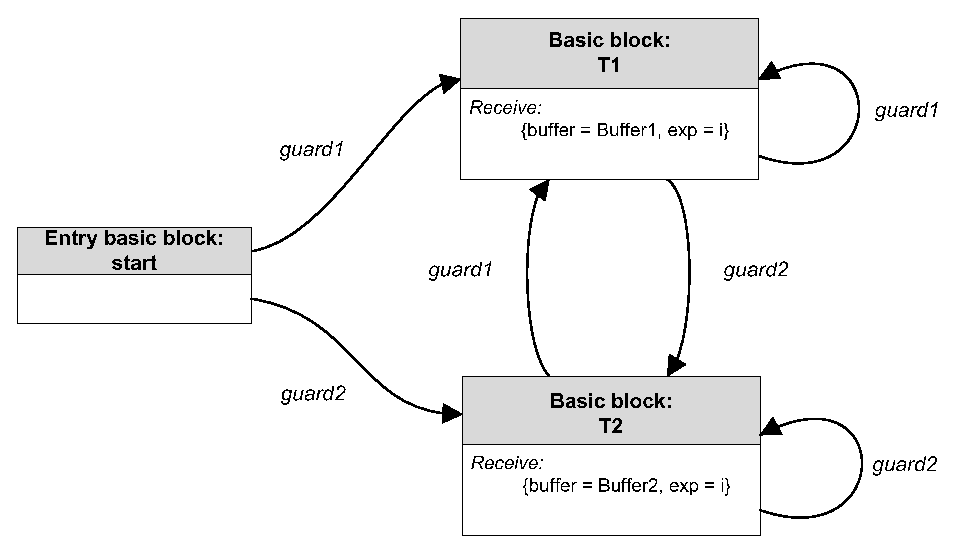
\includegraphics[scale=0.5]{translation/advancedissues/graphics/cffcfg.eps}
\caption{The CFG showing the control flow branch}
\label{fig:cffcfg}
\end{figure}

\subsubsection{Translating to an AST}

The CFG is then translated to the AST shown in Fig.~\ref{fig:cffast}. The \code{Process} node contains two blocks \code{T1} and \code{T2}. Taking a look at \code{T1} it contains a receive statement which has a pointer to \code{Buffer1} where the incoming messages are stored. The receive statement also contains a local variable \code{i} into which a message from the buffer is read. \code{T1} also contains two conditional statements; one holding the condition expression \code{guard1} and pointing to \code{T1}, and one holding the condition expression \code{guard2} and pointing to \code{T2}. The block \code{T2} is similar to \code{T1}.

\begin{figure}[b!]
\centering
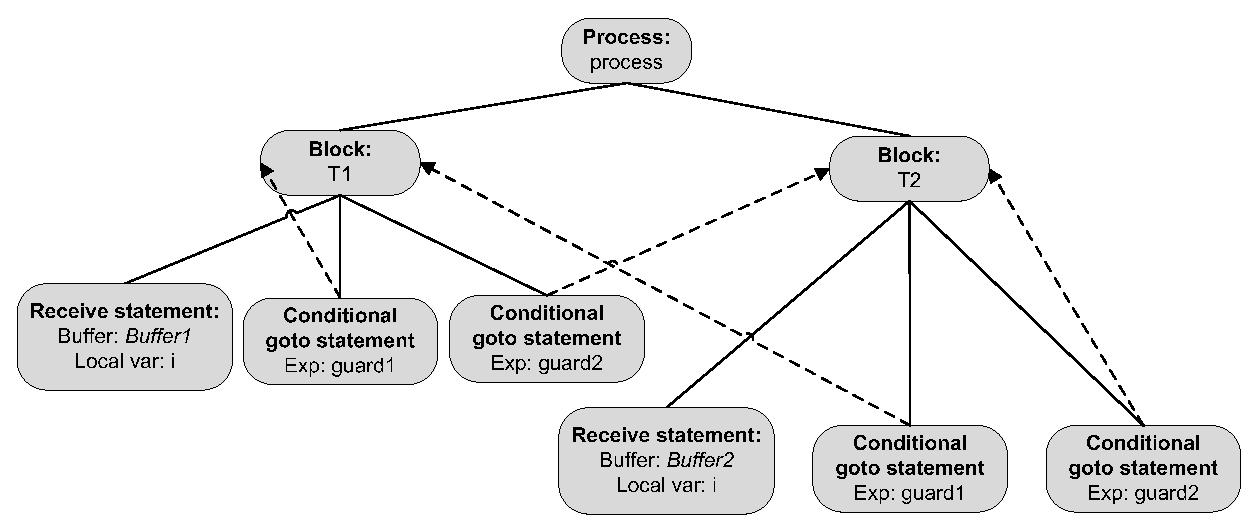
\includegraphics[scale=0.65]{translation/advancedissues/graphics/cffast.eps}
\caption{The AST showing the control flow branch}
\label{fig:cffast}
\end{figure}

\subsubsection{Translating to Erlang Source Code}
%In the phase from AST to EST things become a bit more complicated when buffers are involved as in this small example.
Next, we explain how control flow branches are handled when there are no buffers involved. In this section we omit the EST and only show the printed Erlang code. In Listing~\ref{list:cffnobuf} we see the code for \code{t1} generated from the AST (ignoring the receive statements) in Fig.~\ref{fig:cffast}.

\begin{figure}[h!]
\begin{verbatim}[style=erlangcode, caption=Generated Erlang code without receive statements, label=list:cffnobuf]
t1() -> 
    ...
    if
        Guard1 ->
            t1();
        Guard2 ->
            t2()
    end.
\end{verbatim}
\end{figure}


In the bottom of the function the guard expressions are evaluated, and jumps are made accordingly. Notice that if none of the guard expressions evaluate to \code{true} the program terminates. This is equivalent to the behaviour of the CPN model, in which this corresponds to none of the transitions, the process can proceed to, being enabled. Since we do not allow tokens on shared places or buffer places to be referred to in the guard expressions, the transitions cannot become enabled in the future.

This is code is generated for control flow branches when the goto statements points to blocks without receive statements. Generating Erlang code when there is a receive statement in one of the target blocks is a bit more complicated.

\paragraph{Goto a block with a receive statement.}
Jumping to the first block were the guard evaluates to \code{true} could introduce a deadlock in the program if that block contains a receive statement from a buffer that will never have an element added. For instance, in the ProPCPN model shown in fig.~\ref{fig:cffcpn}, it could be the case that both \figitem{guard1} and \figitem{guard2} evaluates to \code{true}. Assume that \figitem{Buffer1} is empty, and that there will never be added a token to it. Assume also that \figitem{Buffer2} already contains a token. If the program where to jump to the function corresponding to the transition \figitem{T1} the program would stop on the blocking receive expression. This is not desirable since \figitem{T2} is enabled in the CPN model, thus calling the function corresponding to \figitem{T2}, would not make the program stop.

The solution we have found is to only jump to a function with a receive expression if there is an element in the buffer. Since buffers are local to a process instance, the element will remain in the buffer until removed by that process instance. Thus it is guaranteed that the buffer element is still available when the function will be executed. We have introduced an explicit Erlang buffer module (found in appendix \ref{appsec:buffer}) with two additional operations:

\begin{itemize}
 \item The function \code{has\_element} can be used to determine if there is an element in the buffer. It does not change the state of the buffer. 
 \item The function \code{interrupt\_me} is used like a blocking receive call if the buffer is empty. The buffer will send a message with the atom literal \code{interrupt} when an element is added to the buffer.
\end{itemize}

\begin{figure}[h!]
\begin{verbatim}
    t1(Env) -> 
    ...
    t1_loop(Env).

t1_loop(Env) -> 
    Env#environment.buffer_1 ! has_element,
    receive 
        Buffer_1_has_elements -> 
            Buffer_1_has_elements
    end,
    Env#environment.buffer_2 ! has_element,
    receive 
        Buffer_2_has_elements -> 
            Buffer_2_has_elements
    end,
    if
        Guard1, Buffer_1_has_elements ->
            t1(Env); 
        Guard2, Buffer_2_has_elements ->
            t2(Env);
        true ->
            if
                not Buffer_1_has_elements ->
                    Env#environment.buffer_1 ! interrupt_me;
            end,       
            if       
                not Buffer_2_has_elements ->
                    Env#environment.buffer_2 ! interrupt_me
            end
    end,
    receive 
        interrupt -> 
            t1_loop(Env)
    end.
\end{verbatim}
\end{figure}


Listing~\ref{list:cffwithbuf} shows how \code{has\_element} and \code{interrupt\_me} are used in the generated code. The function \code{t1\_loop} line 5-34 is used to decide which function to call next. In line 6-15 the \code{has\_element} operation is used on \code{Buffer1} and \code{Buffer2} and bound to variables. In line 17-18 we see how the function \code{t1} is called if \code{Guard1} evaluates to \code{true} and the buffer has an element. The \code{true} branch in line 21-29 is used if no function is available, i.e., none of the above guards evaluates to \code{true} or the buffers had no elements. This means, that until one of the buffers receives an element, none of the functions can be called. For this reason, it is requested that all the buffers without elements make an interrupt when an element becomes available. Finally, in line 31-34 \code{t1} is blocked until an interrupt is received from one of the buffers, in which case \code{t1\_loop} is called again.
